%!TEX root = ../thesis.tex
% ******************************* Thesis Appendix B ********************************

\chapter{Simulated Cosmic $\mu$ Tomographic Outlines}

\begin{sidewaysfigure}[htbp]
 \centering
 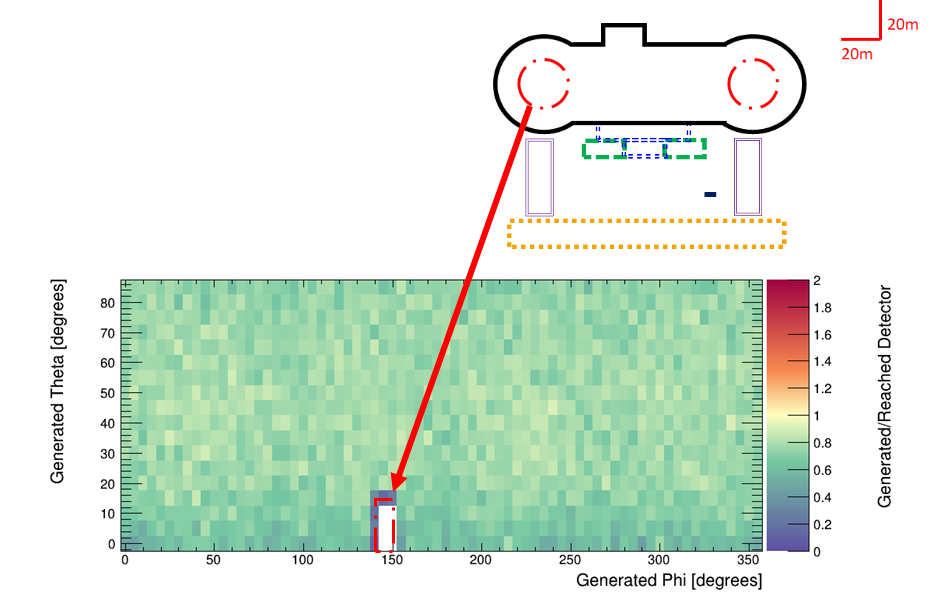
\includegraphics[width=\linewidth]{Chapter5/Figs/wylfaRasterNew/reactorCoreFarGen_Reached.png}
 \captionof{figure}{How the outline for the reactor far from the detector looks in simulation to our detector.} 
 \label{fig:reactorCoreFarGen_Reached}
\end{sidewaysfigure}

\begin{sidewaysfigure}[htbp]
 \centering
 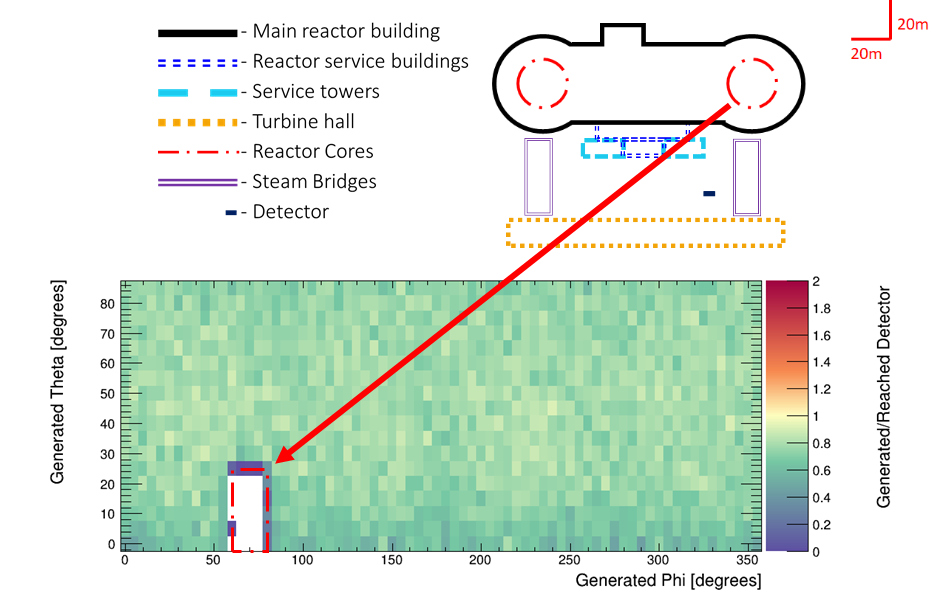
\includegraphics[width=\linewidth]{Chapter5/Figs/wylfaRasterNew/reactorCoreNearGen_Reached.png}
 \captionof{figure}{How the outline for the reactor close to the detector looks in simulation to our detector} 
 \label{fig:reactorCoreNearGen_Reached}
\end{sidewaysfigure}

\begin{sidewaysfigure}[htbp]
 \centering
 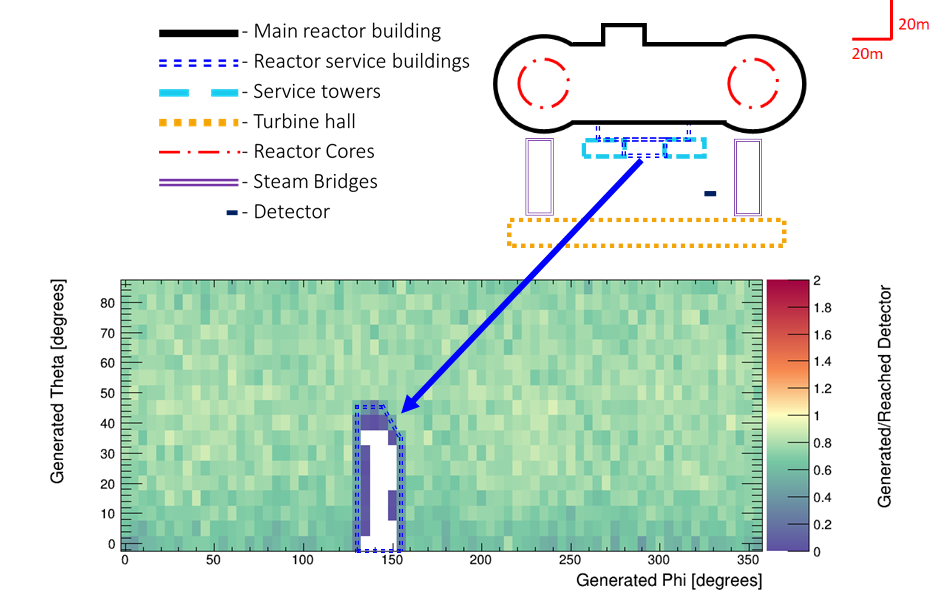
\includegraphics[width=\linewidth]{Chapter5/Figs/wylfaRasterNew/serviceBuildClose.png}
 \captionof{figure}{How the service building closest to the detector looks in simulation.} 
 \label{fig:serviceBuildClose}
\end{sidewaysfigure}

\begin{sidewaysfigure}[htbp]
 \centering
 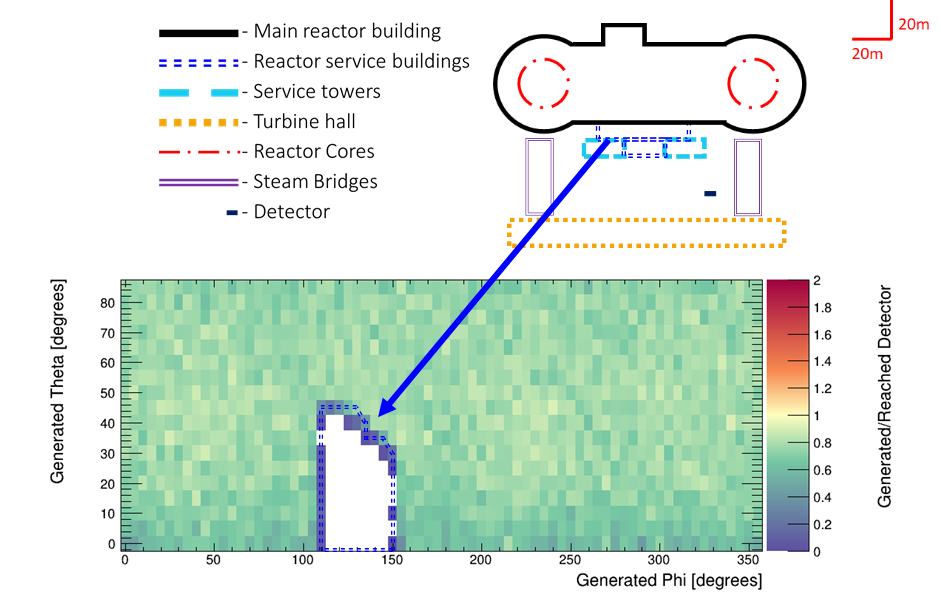
\includegraphics[width=\linewidth]{Chapter5/Figs/wylfaRasterNew/serviceBuildFar.png}
 \captionof{figure}{How the service building furthest from the detector looks in simulation.} 
 \label{fig:serviceBuildFar}
\end{sidewaysfigure}

\begin{sidewaysfigure}[htbp]
 \centering
 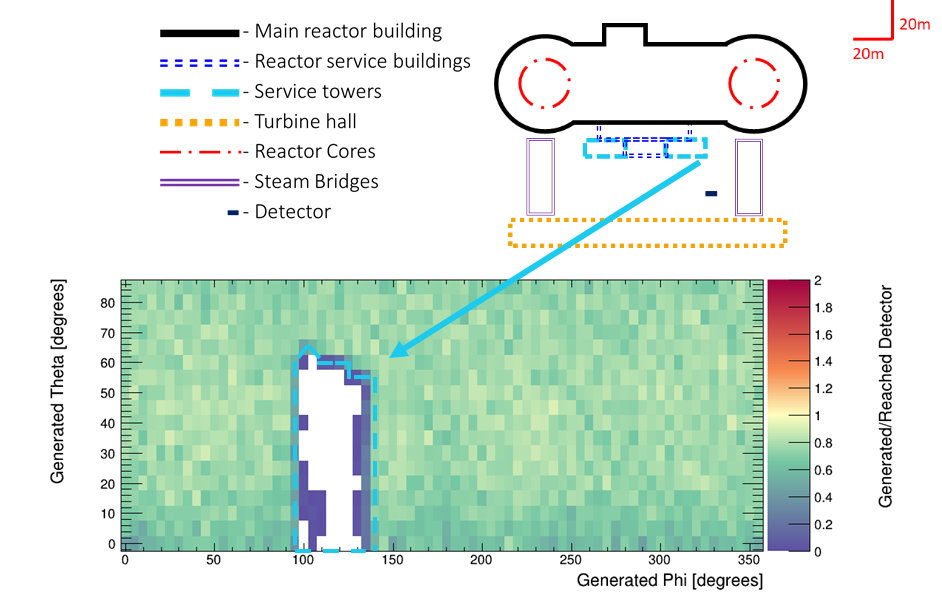
\includegraphics[width=\linewidth]{Chapter5/Figs/wylfaRasterNew/serviceTowerCloseGen_Reached.png}
 \captionof{figure}{How the service tower close to the detector looks in simulation.} 
 \label{fig:serviceTowerCloseGen_Reached}
\end{sidewaysfigure}

\begin{sidewaysfigure}[htbp]
 \centering
 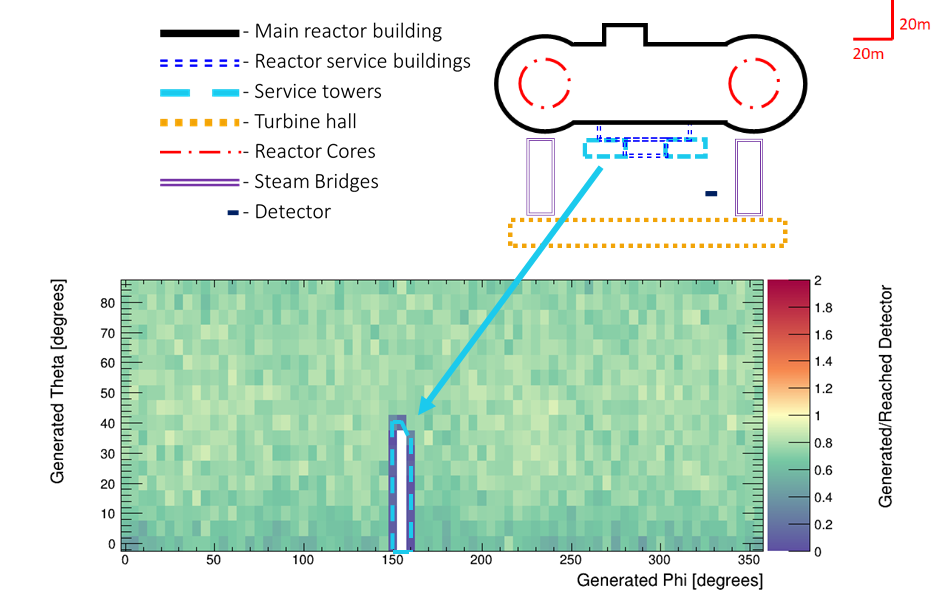
\includegraphics[width=\linewidth]{Chapter5/Figs/wylfaRasterNew/serviceTowerFarGen_Reached.png}
 \captionof{figure}{How the service tower furthest from the detector looks in simulation.} 
 \label{fig:serviceTowerFarGen_Reached}
\end{sidewaysfigure}

\begin{sidewaysfigure}[htbp]
 \centering
 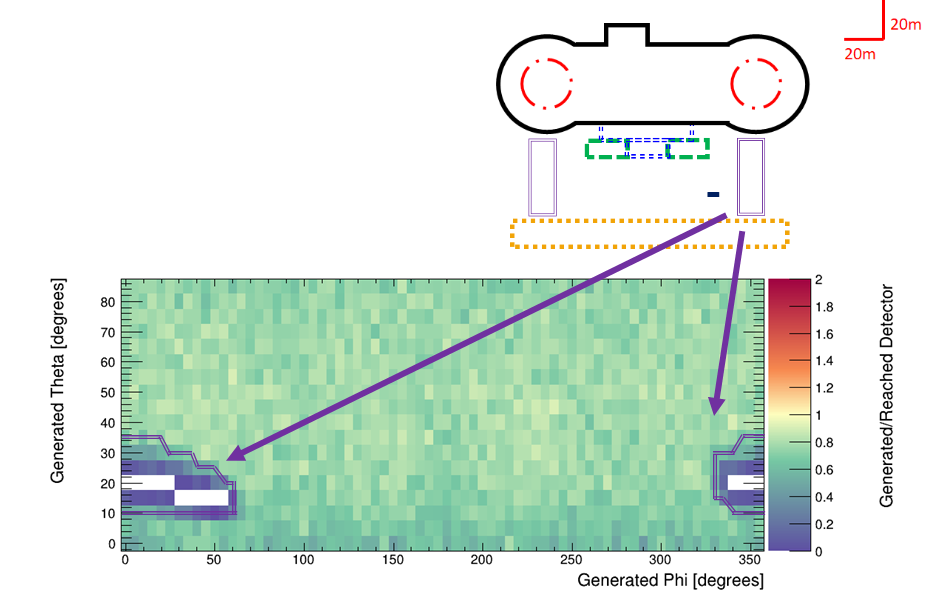
\includegraphics[width=\linewidth]{Chapter5/Figs/wylfaRasterNew/steamBridgeCloseGen_Reached.png}
 \captionof{figure}{How the steam bridge closest to the detector looks in simulation.} 
 \label{fig:steamBridgeCloseGen_Reached}
\end{sidewaysfigure}

\begin{sidewaysfigure}[htbp]
 \centering
 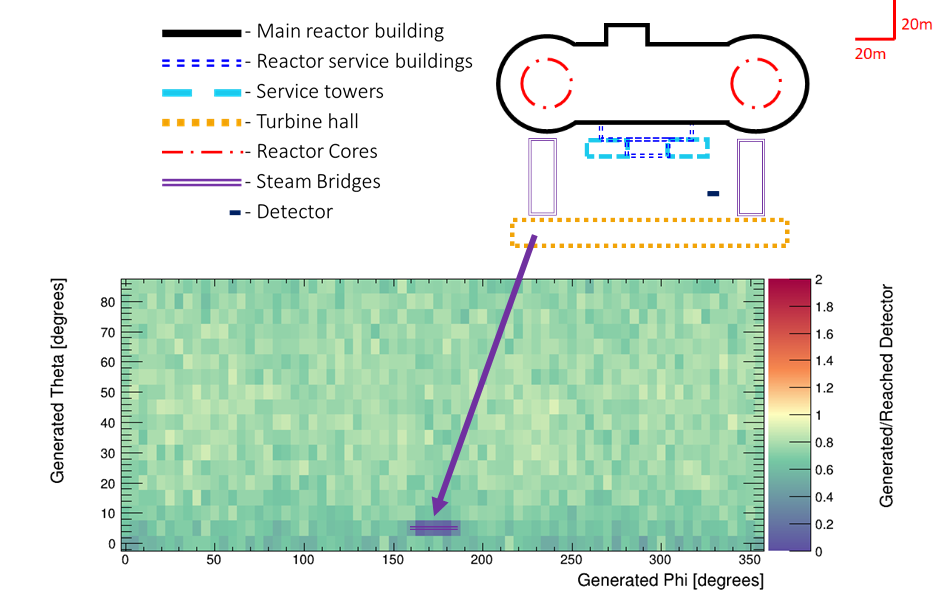
\includegraphics[width=\linewidth]{Chapter5/Figs/wylfaRasterNew/steamBridgeFarGen_Reached.png}
 \captionof{figure}{How the steam bridge furthest from the detector looks in simulation.} 
 \label{fig:steamBridgeFarGen_Reached}
\end{sidewaysfigure}

\begin{sidewaysfigure}[htbp]
 \centering
 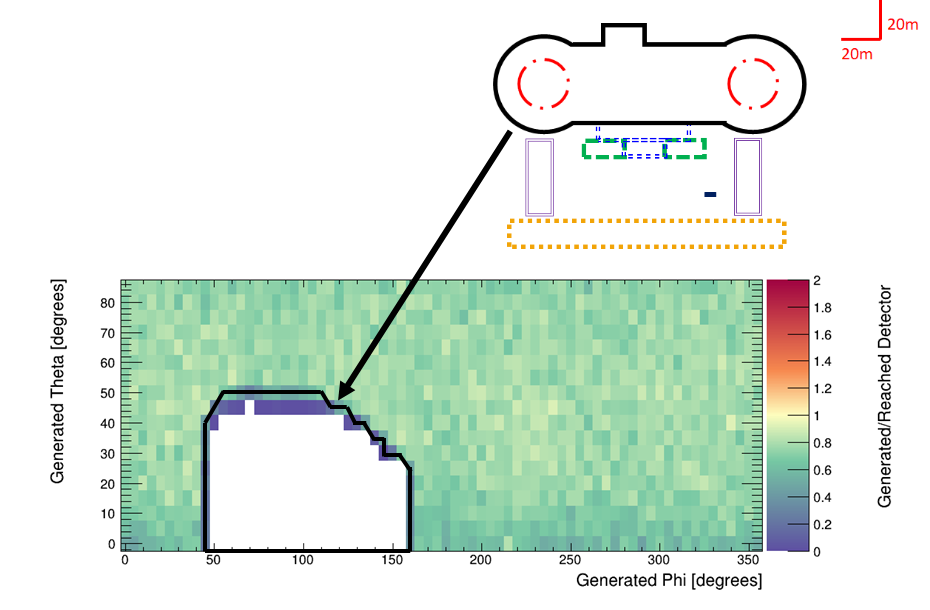
\includegraphics[width=\linewidth]{Chapter5/Figs/wylfaRasterNew/dogBoneGen_Reached.png}
 \captionof{figure}{How the main ``dog bone'' structure of the main reactor building looks in simulation.} 
 \label{fig:dogBoneGen_Reached}
\end{sidewaysfigure}

\begin{sidewaysfigure}[htbp]
 \centering
 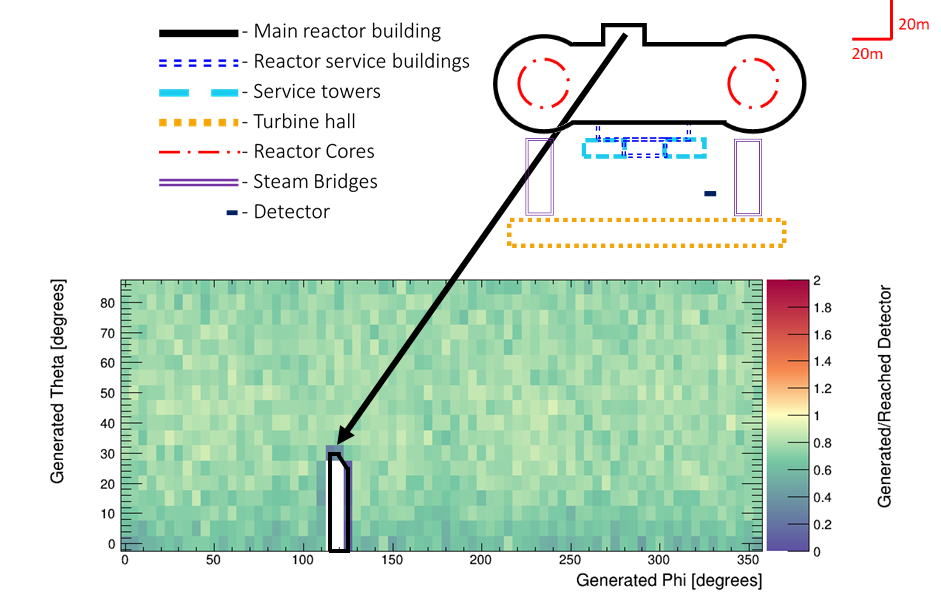
\includegraphics[width=\linewidth]{Chapter5/Figs/wylfaRasterNew/backServiceGen_Reached.png}
 \captionof{figure}{How the back service building of the main reactor building looks in simulation.} 
 \label{fig:backServiceGen_Reached}
\end{sidewaysfigure}

\begin{sidewaysfigure}[htbp]
 \centering
 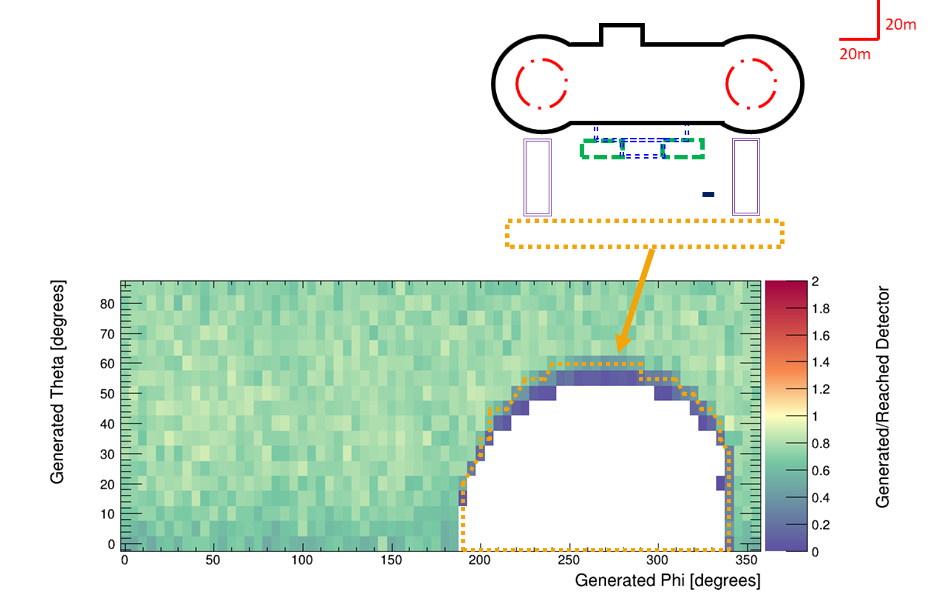
\includegraphics[width=\linewidth]{Chapter5/Figs/wylfaRasterNew/TurbineHallGen_Reached.png}
 \captionof{figure}{How the turbine hall looks in simulation.} 
 \label{fig:TurbineHallGen_Reached}
\end{sidewaysfigure}


% \LaTeX.cls files can be accessed system-wide when they are placed in the
% <texmf>/tex/latex directory, where <texmf> is the root directory of the user’s \TeX installation. On systems that have a local texmf tree (<texmflocal>), which
% may be named ``texmf-local'' or ``localtexmf'', it may be advisable to install packages in <texmflocal>, rather than <texmf> as the contents of the former, unlike that of the latter, are preserved after the \LaTeX system is reinstalled and/or upgraded.

% It is recommended that the user create a subdirectory <texmf>/tex/latex/CUED for all CUED related \LaTeX class and package files. On some \LaTeX systems, the directory look-up tables will need to be refreshed after making additions or deletions to the system files. For \TeX Live systems this is accomplished via executing ``texhash'' as root. MIK\TeX users can run ``initexmf -u'' to accomplish the same thing.

% Users not willing or able to install the files system-wide can install them in their personal directories, but will then have to provide the path (full or relative) in addition to the filename when referring to them in \LaTeX.